% !TEX root = dissertation_BB.tex
%% spellcheck-language en-US

%  ####
%      #
%   ###
%      #
%  ####

\section{Image processing for multi-view microscopy}
  \graphicspath{{./figures/3_processing/}}

  When using any kind of microscopy in research, image processing is a crucial part of the workflow. This is especially true for light-sheet microscopy, since it's capable imaging the same specimen for multiple days, producing immense amounts of data. A single overnight experiment of \textit{Drosophila} development (which is a very typical use-case for light-sheet) can produce multiple terabytes of data. To see the real scales, let's consider the following imaging conditions:
  \begin{center}
  \begin{tabular}{rl}
      camera & Hamamastu Orca Flash 4 \\
      image size & 8 MB \\
      1 stack = 250 planes & 2 GB \\
      2 views & 4 GB \\
      Time-lapse: 16 h @ 2/min & 7.5 TB \\
      $n$ colors & $n\cdot 7.5$ TB
  \end{tabular}
  \end{center}

  As it is apparent from this table, 
  % proportional to the symbol frequencies. A string of symbols can be encoded by applying this process recursively: The sub-interval from the previous step is subdivided again using the same proportions. Figure4.2. shows an example of arithmetic coding using

      
  \subsection{Registration}
    \subsubsection{Image based registration}
    \subsubsection{Bead based registration}
  \subsection{Transformation}
    \subsubsection{Rigid}
    \subsubsection{Affine}
    \subsubsection{Elastic}
  \subsection{Image fusion}
      \subsubsection{Average}
    \subsubsection{Sigmoidal weighted average}
    \subsubsection{Fourier mixing}
    Huisken had something like this
    \subsubsection{Wavelet-based fusion}
    \subsubsection{Multi-view deconvolution}
    
    \cite{krzic_multiple-view_2009} Uros thesis
    \cite{temerinac-ott_multiview_2012}, \cite{temerinac-ott_spatially-variant_2011} Spatially variant deconvolution



\section{Image compression}
  Image compression is an important tool for everyday life, however it's rarely used in the context of scientific imaging because of fear of information loss. This preconception is mainly due to the famous blocking artifacts found in many highly compressed JPEG images, however not all image compression algorithms introduce artifacts, and in fact many lossless algorithms exist that would be suitable for such images. Nowadays, when data production is in an exponential growth compression is again in highlight, without it it would be extremely difficult to maintain many scientific projects that produce images at a high data rate. 

  In this paper I will review the basics of image compression based on Sayood's textbook, Introduction to Data Compression \cite{sayood_introduction_2012}. 
  I will introduce some basics of information theory and entropy, followed by discussing two widely used entropy coding algorithms, Huffman coding and arithmetic coding. Section 3 will be about transform coding, specifically Discrete Cosine Transform (DCT) and wavelet transform while also touching upon techniques based on differential pulse code modulation. Finally I will show how some of the most widely used image compression standards use these methods to achieve effective image compression.

  \subsection{Entropy coding}
    \subsubsection{Information and Entropy}
      For the purpose of data compression it is useful to quantify the amount of \textit{information} contained within a piece of data. The first rigorous definition of information was presented in an extremely influential paper by Shannon, published in two parts in 1948 \cite{shannon_mathematical_1948, shannon_mathematical_1948-1}.

      First, let's define the amount of self-information contained in the outcome of a random experiment:
      \begin{equation}
        I(A) = \log_b \frac{1}{P(A)} = - \log_b P(A)
      \end{equation}

      2 independent events:
      \begin{equation}
        P(A,B) = P(A) \cdot P(B)
      \end{equation}

      self-information is additive:
      \begin{align}
        I(A,B) &= \log_b \frac{1}{P(A,B)} \\
        &= \log_b \frac{1}{P(A) \cdot P(B)} \\
        &= \log_b \frac{1}{P(A)} + \log_b \frac{1}{P(B)}
      \end{align}

      entropy for random variable $X$ ~ average or expected self-information for the random variable
      \begin{equation}
        H(X) = \sum_i P(A_i)I(A_i) = - \sum_i P(A_i) \log_b P(A_i)
      \end{equation}

      entropy rate for data source $S$ ~ average information output by the data source

    \subsubsection{Huffman coding}
      Huffman coding is a prefix-free, optimal code that is widely used in data compression. It was developed by David A. Huffman as a course assignment on the first ever course on information theory at MIT, and was published shortly afterwards \cite{huffman_method_1952}. It is a variable length binary code which assigns different length codewords to letters of different probabilities. It is able to achieve optimal compression, which means the total length of the coded sequence will be minimal.

      Although it produces a variable length code which can introduce some issues with decoding, it is still uniquely decodable. It achieves this property by using prefix-free codewords, meaning that none of the codewords are prefixes of any other codewords. This property can be exploited when decoding the codeword, since during this procedure the number of bits for the next codeword can not be determined in advance. However if no codeword is a prefix of another codeword, by simply reading the successive bits one by one until we reach a valid codeword, it's possible to uniquely decode the message.

      Let's take the example in Table \ref{tab:huffman1}. Five letters are coded in binary code by Code \#1 and by Code \#2. Code 1 is not a prefix code, and because of this when reading the encoded sequence we can not be sure when we reach the end of a codeword. Decoding the sequence 0000 for example could be interpreted as 4 letters of $a_1$ or 2 letters of $a_3$.

      \begin{table}
        \bcaption[Examples of a random binary code (\#1) and a prefix-free binary code (\#2)]{Code \#2 is uniquely decodable, while for code \#1 it's necessary to introduce boundaries between codewords to be able to distinguish them.}
        \centering
        \begin{tabular}{crr}
          \toprule
          Letter & Code \#1 & Code \#2 \\
          \midrule
          $a_1$ & 0	& 10 \\
          $a_2$ & 11	& 11 \\
          $a_3$ & 00	& 00 \\
          $a_4$ & 10 	& 010 \\
          $a_5$ & 111	& 011 \\
          \bottomrule
        \end{tabular}
        \label{tab:prefix}
      \end{table}

      The Huffman coding procedure is based on two observations regarding optimal and prefix-free codes:
      \begin{enumerate}
        \item For a letter with higher frequency the code should produce shorter codewords, and for letters with lower frequency it should produce longer codewords.
        \item In an optimum code, the two least frequent codewords should have the same lengths.
      \end{enumerate}

      From these statements the first is trivial to see that is correct. If the more frequent letters would have longer codewords then the less frequent letters, the average codeword length (weighted by the probabilities) would be larger than in the opposite case. Thus, more frequent letters must not have longer codewords than less frequent letter.

      The second statement at first glance might be so intuitive, so let's consider the following situation. The two least frequent codewords do not have the same lengths, that is the least frequent is longer. However, because this is a prefix code, the second longest codeword is not a prefix of the longest codeword. This means, if we truncate the longest codeword to the same length as the second longest, they will still be distinct codes and uniquely decodable. This way we have a new coding scheme which requires less space on average to code the same sequence as the original code, from which we can conclude the original code was not optimal. Therefore, for an optimal code, statement 2 must be true.

      \begin{table}
        \bcaption[Huffman code table]{}
        \centering
        \begin{tabular}{ccr}
          \toprule
          Letter & Probability & Codeword \\
          \midrule
          $a_2$ & 0.4 & $c(a_2)$ \\
          $a_1$ & 0.2 & $c(a_2)$ \\
          $a_3$ & 0.2 & $c(a_2)$ \\
          $a_4$ & 0.1 & $c(a_2)$ \\
          $a_5$ & 0.1 & $c(a_2)$ \\
          \bottomrule
        \end{tabular}
        \label{tab:huffman1}
      \end{table}

      \begin{figure}
        \centering
        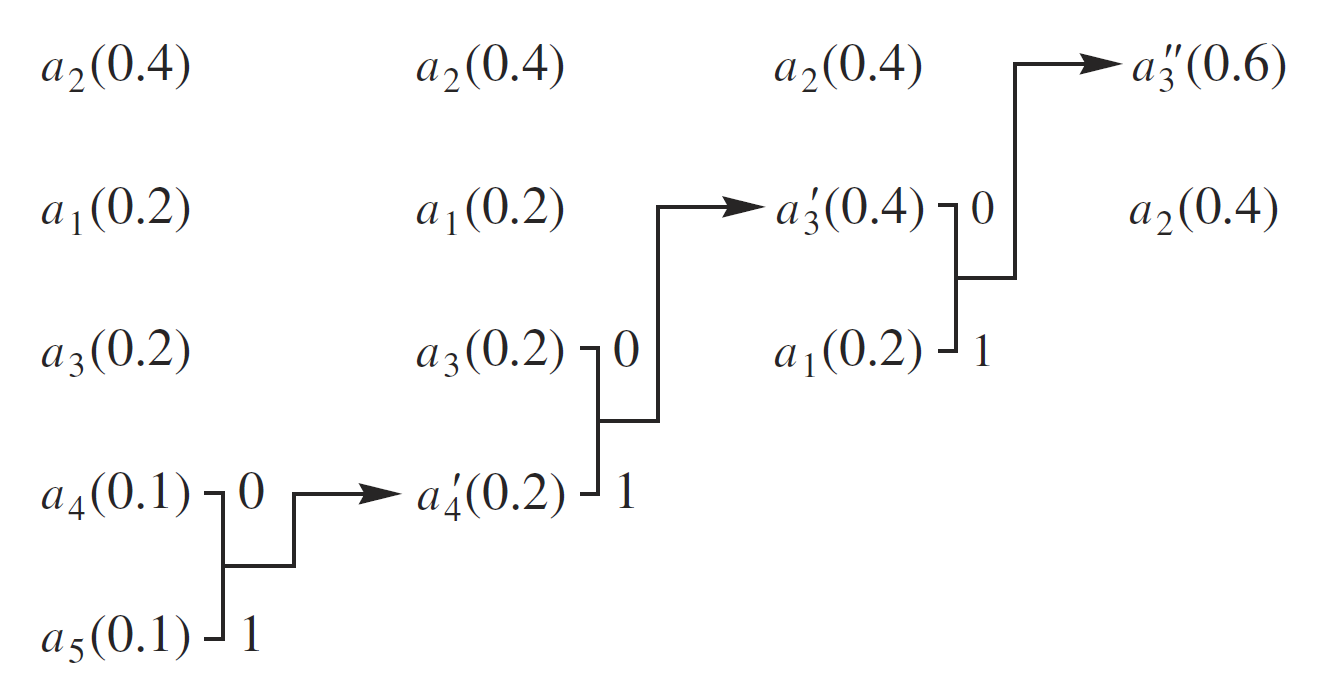
\includegraphics[width=0.6\textwidth]{huffman}
        \bcaption[Building the binary Huffman tree]{The letters are ordered by probability, these will be the final leave of the tree. To join the to branches at every iteration we join the to nodes with the smallest probability, and create a new common node with the sum of the probabilities. This process is continued until all nodes are joined in a root node with probability of 1. Now, if we traverse down the tree to each leaf, the codeword will be defined by their position.}
        \label{fig:huffman}
      \end{figure}

      To construct such a code, the following iterative procedure can be used. Let's consider an alphabet with five letters $A = [a_1,a_2,a_3,a_4,a_5]$ with $P(a_1)=P(a_3)=0.2$, $P(a_2)=0.4$ and $P(a_4)=P(a_5)=0.1$ (Table \ref{tab:huffman1}). The entropy for this source is 2.122 bits/symbol. Let's order the letters by probability, and consider the two least frequent. Since the codewords assigned to these should have the same lengths, we can assign their codewords as
      \begin{align*}
        c(a_4) &= \alpha_1 * 0 \\
        c(a_5) &= \alpha_1 *1
      \end{align*}

      where $c(a_i)$ is the assigned codeword for letter $a_i$ and $*$ denotes concatenation. Now we define a new alphabet $A'$ with only four letters $a_1, a_2, a_3, a'_4$, where $a'_4$ is a merged letter for $a_4$ and $a_5$ with the probability $P(a'_4) = P(a_4) + P(a_5) = 0.2$. We can continue this process of merging the letters until all of them are merged and we have only one letter left. Since this contains all of the original letter, its probability is 1. We can represent the end result in a binary tree (see Figure \ref{fig:huffman}), where the leaves are the letter of the alphabet, nodes are the merged letters, and the codewords are represented by the path from the root node to each leaf (compare with Table \ref{tab:huffman2}). The average length of this code is
      \begin{equation}
        l = 0.4\times 1 + 0.2 \times 2 + 0.2 \times 3 + 0.1 \times 4 + 0.1 \times 4 = 2.2 \text{ bits/symbol}
      \end{equation}
      A measure of the efficiency of this code is its redundancy—the difference between the entropy
      and the average length. In this case, the redundancy is 0.078 bits/symbol. The redundancy is
      zero when the probabilities are negative powers of two.

      \begin{table}
        \bcaption[Huffman code table]{}
        \centering
        \begin{tabular}{ccr}
          \toprule
          Letter & Probability & Codeword \\
          \midrule
          $a_2$ & 0.4 & 1 \\
          $a_1$ & 0.2 & 01 \\
          $a_3$ & 0.2 & 000 \\
          $a_4$ & 0.1 & 0010 \\
          $a_5$ & 0.1 & 0011 \\
          \bottomrule
        \end{tabular}
        \label{tab:huffman2}
      \end{table}


    \subsubsection{Arithmetic coding}
      Although in this case the redundancy of the Huffman code is minimal, however in cases where a few symbols have vary high probability compared to the rest, the redundancy increases. This is simply because even for the most frequent letter the shortest codeword the Huffman code can produce is of length 1.

      Let's consider the following example: take alphabet $A=[a_1, a_2]$ with $P(a_1) = 0.95$ and $P(a_2) = 0.05$. The first order entropy for this source is $-0.95 \log 0.95 - 0.05 \log 0.05 = 0.2864$ bits/symbol, however if we assign the Huffman code we will have to use $c(a_1)=0$ and $c(a_2)=1$, which means the average length will be 1 bit/symbol. This means in order to code this sequence using a Huffman code, we will need more than 3 times the number of bits promised by the entropy.

      To get around this fundamental limitation, a coding scheme must be used which does not use discrete codewords at all. Arithmetic coding is the most well-known example of such a scheme. The idea is due to Peter Elias. He developed it during the same course on information theory in which Huffman developed his coding method, but he never published it.

      In order to distinguish a sequence of symbols from another sequence of symbols we need to
      tag it with a unique identifier. One possible set of tags for representing sequences of symbols
      are the numbers in the unit interval [0,1). Because the number of numbers in the unit interval
      is infinite, it should be possible to assign a unique tag to each distinct sequence of symbols. In
      order to do this, we need a function that will map sequences of symbols into the unit interval.

      A straightforward algorithm to arithmetically encode a given input string is the
      following: Partition the unit interval [0, 1) into sub-intervals and assign one subinterval
      to each symbol in the input alphabet. The sizes of the sub-intervals are
      chosen to be proportional to the symbol frequencies. A string of symbols can be
      encoded by applying this process recursively: The sub-interval from the previous
      step is subdivided again using the same proportions. Figure \ref{fig:arithmetic}. shows an example of
      arithmetic coding using the symbol frequencies given in Table \ref{tab:arithmetic}.

      \begin{table}
        \bcaption[Example alphabet for arithmetic coding]{}
        \centering
        \begin{tabular}{cc}
          \toprule
          Letter & Probability \\
          \midrule
          $a_1$ & 0.7 \\
          $a_2$ & 0.1 \\
          $a_3$ & 0.2 \\
          \bottomrule
        \end{tabular}
        \label{tab:arithmetic}
      \end{table}

      \begin{figure}
        \centering
        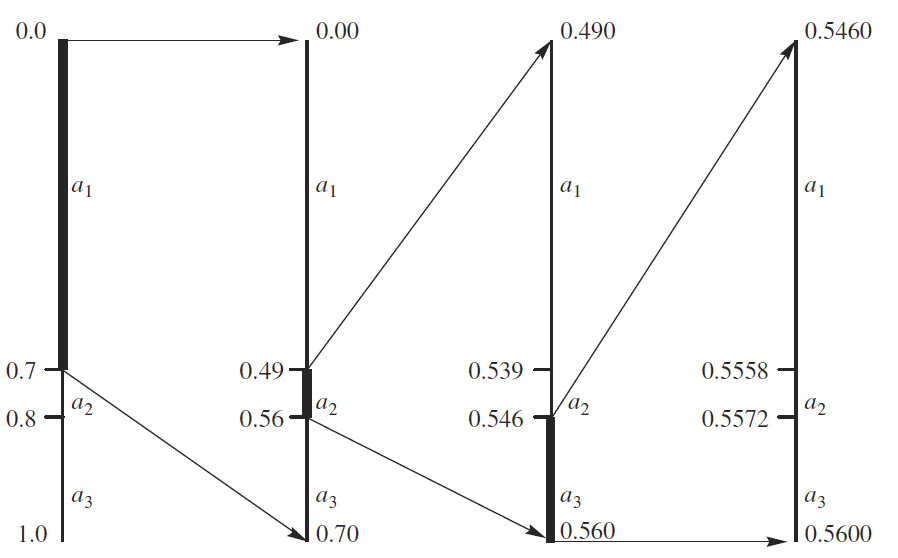
\includegraphics[width=0.6\textwidth]{arithmetic}
        \bcaption[Arithmetic coding scheme in practice with the alphabet from Table \ref{tab:arithmetic} on the sequence $a_1,a_2,a_3$]{}
        \label{fig:arithmetic}
      \end{figure}

      This kind of coding although easy to understand, it's actually quite cumbersome to directly implement on a computer, where only a certain floating point precision can be achieved. For real life use this precision is often unsatisfactory, so some extra steps are involved in the coding.

      Since after each step the next subinterval is a subset of the previous interval, if the coding interval after a certain number of steps is contained in either the upper or lower half of the unit interval it will remain there for the rest of the coding. We can exploit this fact by rescaling that interval to the unit interval and writing either a 0 or 1 bit to the output depending on the position of the subinterval. By continuing this scheme it's possible to reach arbitrary precision even using a computer.

      The decoding process is analogous to encoding. The decoder keeps track of the current lower and upper bounds. It mimics the rescaling operations of the encoder based on the bits of the encoded binary number.

  \subsection{Transform coding}
    The methods outlined in the previous section are effective at compressing the data in an optimal way and reaching the first order entropy, however the assume nothing about the structure of the data. For image compression it's important to also consider this, since most images have a relatively high level of autocorrelation, meaning that neighboring values have a high chance of being similar, although not necessarily equal. Transform coding is a technique that by itself does not compress the data, however by exploiting some knowledge of the structure it transforms the data effectively reducing it's first order entropy. When regular entropy coding is then preformed on the transformed data, because of the reduced first-order entropy, these techniques can achieve a higher rate of compression. At decompression, after decoding the entropy coder, the reverse transformation is applied to reveal the original data. In this section I will introduce two of the most important algorithms for transform coding, Discrete Cosine Transform and Wavelet Transform.

    \subsubsection{Discrete Cosine Transform}
      Discrete Cosine Transform \cite{ahmed_discrete_1974} is closely related to the well known Fourier transform. The main idea behind this is to represent a function by a weighted sum of different sine and cosine functions. This provides a different view, instead of looking at the data in the time domain, we gain information about the frequencies that compose the signal. 

      Discrete Cosine Transform is a variant of the discrete Fourier transformation, however instead of making the signal periodic which can introduce large jumps at the edges, the signal is extended in a symmetric way. Since this will give a smooth transition even at the boundaries, the transform does not have to include so many high frequency components. Also, because of the symmetric extension, it's possible to represent the functions only by using the cosine bases, resulting in fewer coefficients. Overall, the DCT is much better suited for compression, than DFT.

      The DCT base functions are defined in the following way:
      \begin{equation}
      c_{i,j} = s_i \cdot \cos \frac{(2j+1)i\pi}{2n} \qquad \text{with } s_i = 
          \begin{cases}
            \sqrt{\frac{1}{n}} & \text{if } i=0 \\
            \sqrt{\frac{2}{n}} & \text{otherwise}
          \end{cases}
      \end{equation}
      The scaling factors is are chosen so that the $L_2$ norm of each basis vector is 1 and
      so the transform is orthonormal. The inverse transform can therefore be found by
      simply transposing the transform matrix.

      \begin{figure}
        \centering
        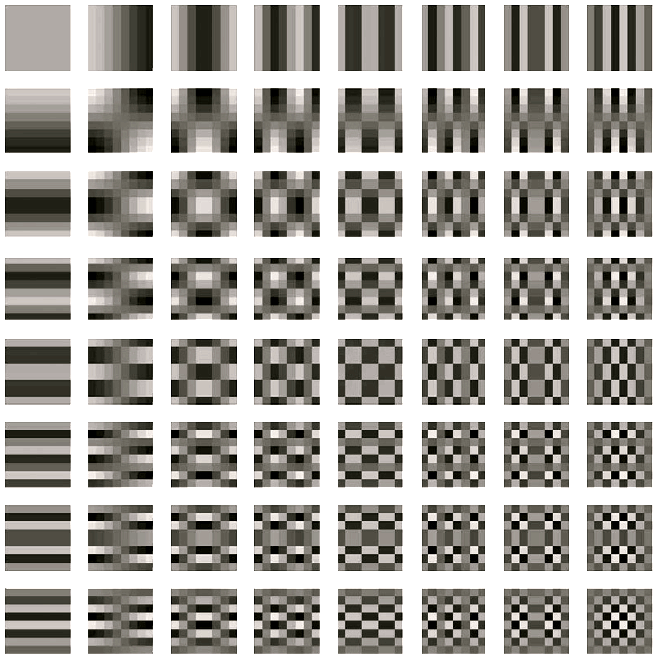
\includegraphics[width=0.4\textwidth]{DCT_bases}
        \bcaption[Basis functions of the $8 \times 8$ 2D DCT, computed as the outer product of the 1D basis vectors.]{}
        \label{fig:DCT_bases}
      \end{figure}

      Applying the DCT to two dimensional functions, i.e. images is very similar to the two dimensional Fourier transform. The base functions are the outer products oft the 1D base functions (Figure \ref{fig:DCT_bases}.), and the transform can actually be performed separately for each dimension.

      Computation effort in a naive implementation is $O(n^2)$ but since DCT is based on the Fourier transform, an $O(n \log n)$ algorithm is also possible, analogous to the fast Fourier transform. This is still larger than a linear scaling with the data size, which can be very inconvenient. Therefore, in practice the DCT is usually applied to smaller blocks of the image, such as $4\times4$, $8\time8$ or $16\times16$. 

      Although DCT is an effective way of reducing the first-order entropy, it has a potential shortcoming by its use of floating point arithmetic. Because of the finite machine precision inherent rounding errors will occur, which means the reverse transformation can not generate the exact original data. For many application, such as photography, this still can be acceptable, but for scientific image data lossy compression is generally not accepted.


    \subsubsection{Discrete Wavelet Transform}
      Methods based on Fourier analysis, such as the DCT introduced in the previous section, give excellent localization in frequency space: They tell us exactly which frequencies occur in the data, which is very useful for data compression. However, they give no spatial localization: They do not tell us where in the signal these frequencies occur. Every DCT base function affect the whole image domain, which means distinct local structures can have a global effect on the final outcome. In case of an edge for example, it's necessary to include a high frequency component with a large coefficient, but since every DCT base function has an impact on the whole domain, this will have to be compensated on smoother regions by also increasing the coefficients of other factors. This can negatively impact compression performance.

      A solution for this is to use different base functions, namely ones with finite support. This way we will not only be able to get information about the frequency, but also about the localization of that frequency in some extent.

      One option for such a set of local basis functions, and certainly the most popular one, is the multi-resolution analysis based on wavelets. The term “multi-resolution analysis” in the context of wavelets was introduced in the late 1980s by Stéphane Mallat \cite{mallat_theory_1989}, though research on wavelets had been ongoing for several years before that.

      The idea behind the wavelet multi-resolution analysis is to build a basis out of translated and scaled versions of one underlying function called the \textit{mother wavelet} $\psi$. The mother wavelet is non-zero only in a small region, leading to the locality properties. It is translated to cover the whole domain. It also covers only a small frequency band, and is scaled to cover higher or lower frequencies. The family of translated and scaled functions $\psi_{l,i}$ is generated from   according to
      \begin{equation}
        \psi_{l,i}(t) = \sqrt{2^l} \psi \left(2^l t-i\right), \qquad l, i \in \mathbb{Z}
      \end{equation}
      Incrementing $l$ halves the width of the resulting function, which thus corresponds to a higher frequency band. Changing $i$ moves the function along the x axis. The size of each step scales with the width of the function, defined by $l$. The normalization factor $\sqrt{2^l}$ is chosen so that the $L_2$ norm stays constant. The mother wavelet can be chosen so that the $\psi_{l,i}$ are pairwise orthogonal and thus form a basis of some function space. However, representing a function in this basis will generally require an infinite number of basis functions $\psi_{l,i}$: To represent a constant component, i.e. content of frequency zero, the wavelet must be infinitely scaled. To address this, it is necessary to introduce an additional scaling function $\phi$ which complements the wavelet. It is scaled and translated the same way as the mother wavelet.

      The oldest wavelets are the Haar wavelets, and because of their simplicity, they provide a good example on how wavelet transformation works. The Haar wavelet scaling $\phi$ and wavelet $\psi$ functions are the following:
      \begin{equation}
        \phi(t) = 
        \begin{cases}
          1 & \text{if } 0 \leq t < 1 \\
          0 & \text{otherwise}
        \end{cases}
        \label{eq:scaling}
      \end{equation}

      \begin{equation}
        \psi(t) = 
        \begin{cases}
          -1 & \text{if } 0 \leq t < \frac{1}{2} \\
          1 & \text{if } \frac{1}{2} \leq t < 1 \\
          0 & \text{otherwise}
        \end{cases}
        \label{eq:wavelet}
      \end{equation}
      Clearly, all wavelet functions $\psi_{l,i}$ are orthogonal. Additionally, the scaling functions $\phi_{l,i}$ at a fixed level $i$ are orthogonal. The scaling functions $\phi_{l,i}$ are also orthogonal to the wavelet functions $\psi_{k,i}$, $k \geq l$ at the same and all finer levels.

      Figure \ref{fig:wavelet}. (left) schematically shows the decomposition of a signal into low-pass components corresponding to the scaling function, and high-pass components corresponding to the wavelet. The signal $s_0$ can be represented by the translated scaling function at a finer scale $l_0$, which can be decomposed to the sum of a coarser approximation $s_1$ corresponding to the scaling function and the detail part $d_1$ corresponding to the wavelet functions. This decomposition to a sum of coarser approximation and detail can be continued multiple times, thus resulting in the previously mentioned multi-resolution analysis.


      \begin{figure}
        \centering
        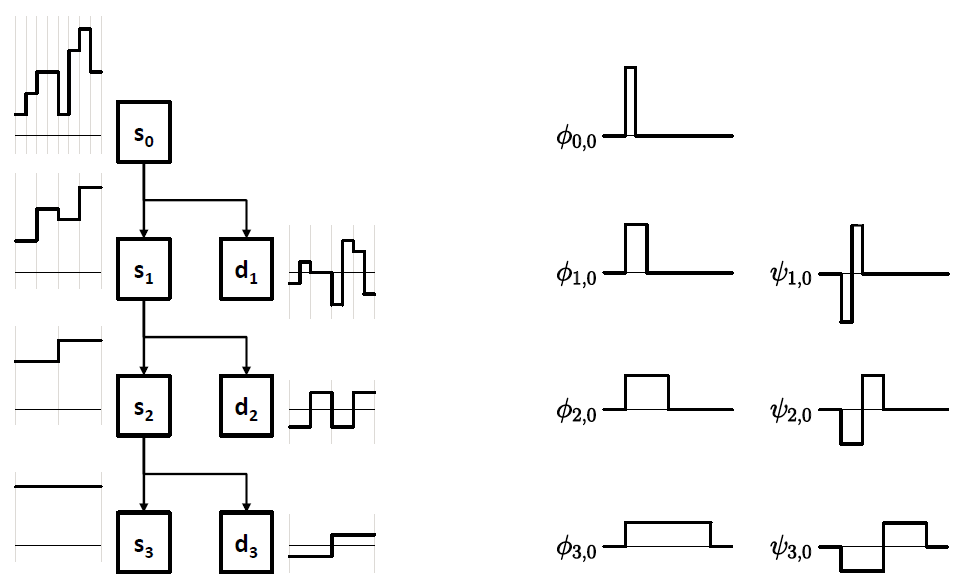
\includegraphics[width=0.6\textwidth]{wavelet}
        \bcaption[Multi-resolution wavelet decomposition, using the Haar wavelets as an example]{Left: decomposition to multiple levels of low pass and high pass coefficients corresponding to the scaling and the wavelet functions respectively. Right: some of the base wavelet functions used for the decomposition.}
        \label{fig:wavelet}
      \end{figure}


      Of course, for image compression applications, it is desirable to extend this transformation to a 2D version, that can be applied to the images before performing the arithmetic coding. Similarly to the DCT, the wavelet transform is also separable, and can be performed as a sequence of 1D transforms along different directions. Separable in a sense, that it does not matter in which order the individual 1D DWTs are applied to get the same 2D transformation.

      JPEG \cite{pennebaker_jpeg:_1992}, JPEG-LS \cite{weinberger_loco-i_2000} and JPEG2000

  \subsection{Differential pulse code modulation / LOCO-I?}

  

  % \section{Conclusion}
  % In this paper I have introduced some of the most important techniques for image compression. Many of these are used in different image compression algorithms, such as . The common point for each of these formats is that they first transform the images to effectively reduce first order entropy, either by predicting the pixel values and coding only the differences (JPEG-LS), or by using either Discrete Cosine Transform (JPEG) or Discrete Wavelet Transform (JPEG2000). In the case of lossy standards after this transformation step a quantization is also performed depending on the desired quality setting for the coder. Finally as the last step the transformed and quantized coefficients are compressed by an arithmetic coder, such as Huffman coding in JPEG of arithmetic coding in JPEG2000. The end result in each case is a highly optimized compression that greatly reduces the file size.

